\documentclass[
BCOR0.7cm,							% Bindekorrektur, bspw. 1 cm
]
{scrbook}

\newif\ifpdf
\ifx\pdfoutput\undefined
	\pdffalse              	%normales LaTeX wird ausgef�hrt
\else
	\pdfoutput=1           
	\pdftrue               	%pdfLaTeX wird ausgef�hrt
\fi

\ifpdf
	%\usepackage{ae}        % Benutzen Sie nur
	%\usepackage{zefonts}  	% eines dieser Pakete
\else
	%%Normales LaTeX - keine speziellen Fontpackages notwendig
\fi

\ifpdf %%Einbindung von Grafiken mittels \includegraphics{datei}
	\usepackage[pdftex]{graphicx} %%Grafiken in pdfLaTeX
\else
	\usepackage[dvips]{graphicx} %%Grafiken und normales LaTeX
\fi


\ifpdf
	\pdfinfo
	{
    /Author (Andreas �sterreicher)                                
    /Title (Testtool-Handbuch)     
    /Subject (Benutzerhandbuch Testtool)                                    
    /Keywords (FH-Complete Technikum-Wien)
	}
\else			
\fi

\usepackage{listings} \lstset{numbers=left, numberstyle=\tiny, numbersep=5pt}
\lstset{language=tex} 
\usepackage{color}
\definecolor{linkfarbe}{rgb}{0.5,0.5,0.5}
\usepackage[pdftex,colorlinks=true,urlcolor=linkfarbe,linkcolor=linkfarbe]{hyperref}
\usepackage[ngerman]{babel}		
\usepackage[T1]{fontenc}
\usepackage[latin9]{inputenc}
\usepackage{makeidx}
\usepackage{float}
\usepackage[small,bf]{caption}
\usepackage{fancyhdr}
\usepackage{amssymb,amsmath}
\makeindex

\graphicspath{{../../images/}}

\setlength{\parindent}{0pt}
\setlength{\parskip}{1ex plus 0.5ex minus 0.2ex}
\addtolength{\textheight}{2cm}
\addtolength{\headheight}{2pt}
\setlength{\captionmargin}{20pt}
\floatstyle{plain}
\floatname{example}{Example}

\newfloat{example}{hbtp}{loe}[chapter]
\floatplacement{figure}{hbtp}
\floatplacement{table}{htbp}

\newcommand{\dollar}{\char36}

\newenvironment{info}[1]{
    \hspace{-10mm}
    \fbox{
        \begin{minipage}{1cm}
        
\includegraphics[width=1cm]{icon_info}
        \end{minipage}
        \begin{minipage}{14.5cm}
        #1
        \end{minipage}
    }
}

\newenvironment{achtung}[1]{
    \hspace{-10mm}
    \fbox{
        \begin{minipage}{1cm}
        
\includegraphics[width=1cm]{icon_achtung}
        \end{minipage}
        \begin{minipage}{14.5cm}
        #1
        \end{minipage}
    }
}

\newenvironment{halt}[1]{
    \hspace{-10mm}
    \fbox{
        \begin{minipage}{1cm}
        
\includegraphics[width=1cm]{icon_halt}
        \end{minipage}
        \begin{minipage}{14.5cm}
        #1
        \end{minipage}
    }
}

\newenvironment{idee}[1]{
    \hspace{-10mm}
    \fbox{
        \begin{minipage}{1cm}
        
\includegraphics[width=1cm]{icon_idee}
        \end{minipage}
        \begin{minipage}{14.5cm}
        #1
        \end{minipage}
    }
}


\setlength{\unitlength}{1mm}

\newenvironment{markier}[5]{
    
    \thicklines \put(#2,#3){\vector(#4,#5){5}} \thinlines
    \put(#2,#3){\circle*{5}}
    \put(#2,#3){\textcolor{black}{\circle{5}}\makebox(-10,0){\textcolor{white}{#1}}}


}


\hyphenation{gleich-zeitig para-meter}


\begin{document}

\ifpdf
	\DeclareGraphicsExtensions{.pdf,.jpg,.png}
\else
	\DeclareGraphicsExtensions{.eps}
\fi

\pagestyle{fancyplain}
% Titelseite einbinden
%
% Titelseite, Abstrakt, Danksagung und Inhaltsverzeichnis
%
%% eigene Titelseitengestaltung %%%%%%%%%%%%%%%%%%%%%%%%%%%%%%%%%%%%%%%    

\begin{titlepage}
\begin{center}
\vspace*{40mm} \huge Testtool-Handbuch\\
\vspace*{10mm}
\vfill 
\includegraphics[width=130mm]{cis}
	
\large \vfill \textsc{Technikum Wien}\\

Wien, \today
\end{center}
\end{titlepage}


\frontmatter					% Vorspann (z.B. r�mische Seitenzahlen)


\tableofcontents			% Inhaltsverzeichnis
%\listoftables				% Tabellenverzeichnis
%\addcontentsline{toc}{section}{Abbildungsverzeichnis}
\listoffigures				% Abbildungsverzeichnis

\chapter{Vorwort}


\mainmatter						% Hauptteil

%% Kapitel Anfang %%%%%%%%%%%%%%%%%%%%%%%%%%%%%%%%%%%%%%%%%%%%%%%%%

\chapter{Testtool}

Das Testtool ist ein Tool zur Abwicklung der Reihungstests. Es dient dazu, ein Ranking der Interessenten  vorzunehmen, um die Besten dieses Tests als Studenten aufzunehmen.

\chapter {Administrationsseite}

Die Administrationsseite des Testtools kann unter /cis/testttool/admin/index.php erreicht werden. Auf dieser Seite k�nnen die Gebiete und Fragen f�r den Reihungstest verwaltet werden.

\begin{figure}
	\centering
	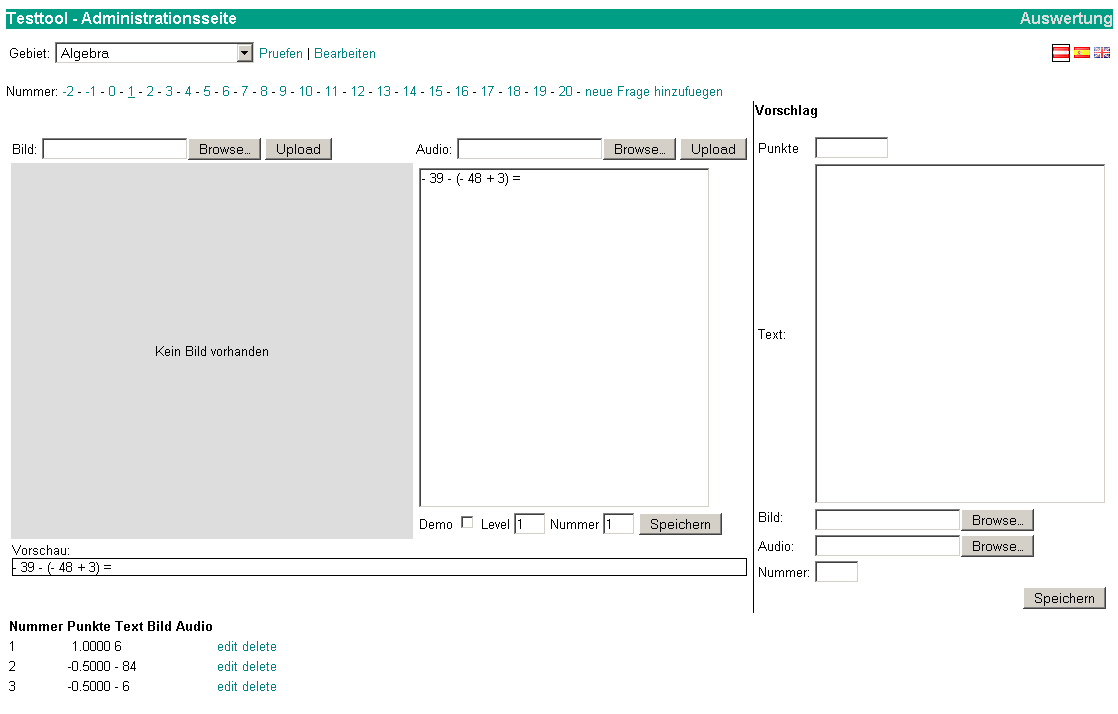
\includegraphics[width=0.75\textwidth]{testtool_admin.png}
	\caption{Testtool-Administration}
	\label{Testtool-Administration}
\end{figure}

\section {Gebiete}

Die Reihungstests k�nnen in unterschiedliche Gebiet aufgeteilt werden (z.B. Algebra, Physik, Englisch, ...)\\
\\
Die folgenden Einstellungen k�nnen bei den Gebieten vorgenommen werden:\\
\\
\begin{itemize}
\item \textbf{Zeit:} Zeit die f�r die Abarbeitung dieses Gebietes zur Verf�gung steht. Format der Eingabe: hh:mm:ss
\item \textbf{Multiple Response:} Wenn diese Option gesetzt ist, k�nnen pro Frage mehrere Antworten gegeben werden.
\item \textbf{Kategorien:} Gibt an ob f�r dieses Gebiet Kategorien vorgesehen sind (nur Pers�nlichkeits-Test)
\item \textbf{Zuf�llige Fragereihenfolge:} Wenn gesetzt, dann werden die Fragen in zuf�lliger Reihenfolge geliefert
\item \textbf{Zuf�llige Vorschlagreihenfolge:} Wenn gesetzt, dann werden die Vorschl�ge in zuf�lliger Reihenfolge geliefert
\item \textbf{Levelgleichverteilung:} Wenn gesetzt, dann wird das Verh�ltnis an Fragen/Level gleich verteilt. Beispiel: sind 6 Fragen des Levels 1 vorhanden und 3 Fragen des Levels 2 und die maximale Fragenanzahl ist 3, dann kommen 2 Fragen mit Level 1 und 1 Frage mit Level 2.
\item \textbf{Maximale Punkteanzahl:} maximal erreichbare Punkte fuer dieses Gebiet. 
\item \textbf{Maximale Fragenanzahl:} maximale Anzahl an erscheinenden Fragen.
\item \textbf{Start Level:} Wenn dieser Wert gesetzt ist, findet ein gelevelter Ablauf statt. 
\item \textbf{Richtige Fragen bis Levelaufstieg:} nur wenn Start Level gesetzt ist; gibt an wie viele Fragen richtig beantwortet werden m�ssen bis der Student einen Level aufsteigt.
\item \textbf{Falsche Fragen bis Levelabstieg:} nur wenn Start Level gesetzt ist; gibt an wie viele Fragen falsch beantwortet werden m�ssen bis der Student einen Level absteigt.
\end{itemize}

\subsection {Einschr�nkungen / Checks:}
\begin{itemize}
\item Wenn ein StartLevel eingetragen wurde, muss eine maximale Fragenanzahl eingetragen werden
\item	Levelgleichverteilung ist nur dann erlaubt, wenn StartLevel nicht gesetzt wurde
\item	Wenn StartLevel gesetzt wurde, muessen von jedem Level mindestens so viele Fragen vorhanden sein wie die "Maximale Fragenanzahl"
\item	Wenn StartLevel gesetzt ist, muessen mindestens 2 unterschiedliche Level vorhanden sein
\item	Wenn Levelgleichverteilung aktiviert ist, muss die maximale Fragenanzahl mindestens so gross sein wie die Anzahl der verschiedenen Level
\item	Wenn Zufallsfrage gesetzt ist und StartLevel oder Levelgleichverteilung gesetzt ist, darf sich die Punkteanzahl pro Level/Frage nicht unterscheiden.
\item	Wenn StartLevel gesetzt ist, darf Multipleresponse nicht gesetzt sein
\item	die Maximale Punkteanzahl muss bei jedem Gebiet eingetragen sein
\end{itemize}
\\
Nachdem ein Gebiet erstellt und mit Fragen bef�llt wurde, kann dieses gepr�ft werden. Dies geschieht �ber den Link 'Pr�fen'. Gebiete k�nnen nur dann im Testtool verwendet werden, wenn das Gebiet Fehlerfrei �berpr�ft werden kann. Ansonsten erscheint das Gebiet w�hrend der Pr�fung in roter Schrift und kann nicht ausgew�hlt werden.\\
\\
Es ist auch m�glich f�r Einsteiger ins 3. Semester eigene Gebiete zu definieren.\\
\\
Eine Zuordnung f�r welchen Studiengang/Semester welches Gebiet angezeigt wird, kann derzeit nur in der Datenbank vorgenommen werden.\\

\section{Fragen}

Wenn ein Gebiet angelegt wurde, k�nnen zu diesem neue Fragen hinzugef�gt werden. Dies geschieht �ber den Punkte 'neue Frage hinzuf�gen'. Die folgenden Attribute k�nnen bei einer Frage eintragen werden:\\

\begin{itemize}
\item \textbf{Bild:} Hier kann ein Bild zu einer Frage hochgeladen werden
\item \textbf{Audio:} Es kann ein Audiofile zu einer Frage hinzugef�gt werden. Die Audio-Files sind als MP3 Mono 11khz 16 Bit hochzuladen.
\item \textbf{Text:} in diesem Fenster kann der Text eingetragen werden der bei der Frage angezeigt wird. Hier k�nnen sowohl Mathematische Formeln mit Hilfe von MathML als auch HTML-Code eingetragen werden. N�here Informationen �ber MathML finden Sie unter http://en.wikipedia.org/wiki/MathML
Im Unteren Teil des Fensters befindet sich ein Vorschaufenster. Dieses zeigt die Vorschau des Textes in Echtzeit an.
\item \textbf{Demo:} Wenn dieses Feld angeklickt wird, erscheint diese Frage vor dem Starten des Gebiets als Demonstrationsbeispiel.
\item \textbf{Level:} gibt den Schwierigkeitsgrad der Frage an. (1=leicht; 5=schwer)
\item \textbf{Nummer:} �ber dieses Attribut wird die Reihenfolge (Sortierung)
 der Fragen bestimmt. Die Nummer von Demo-Fragen sollte kleiner als 0 sein. Die Seite mit der Nummer 0 ist die Startseite f�r das jeweilige Gebiet und sollte eine Kurzbeschreibung oder ein Beispiel des Gebiets enthalten.
\end{itemize}

Die Fragen k�nnen in verschiedene Sprachen �bersetzt werden. Um eine �bersetzung einer Frage anzulegen, klicken Sie einfach auf die entsprechende Sprache im rechten oberen Teil des Fensters.\\

\section{Vorschl�ge}

Pro Frage m�ssen mindestens 2 Vorschl�ge (Antworten) eingetragen werden. F�r jede Antwortm�glichkeit k�nnen Punkte vergeben werden. Es k�nnen auch negative Punkte eingetragen werden, um so einen Punkteabzug bei falschen Antworten zu erm�glichen. \\
\\
Wie bei den Fragen k�nnen auch an die Vorschl�ge Texte, Bilder- und Audio-Dateien angeh�ngt werden.\\
Es muss mindestens eine Frage vorhanden sein, bei der die Punkteanzahl gr��er 0 ist.\\

\chapter{Reihungstest}

Die Seite zum Starten eines Reihungstests findet sich unter /cis/testtool/index.html

\begin{figure}
	\centering
	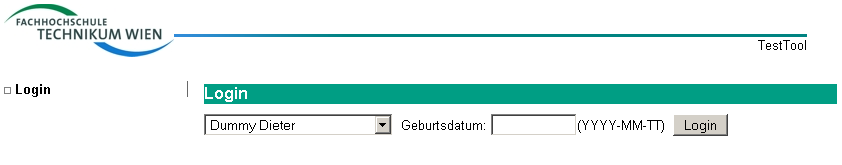
\includegraphics[width=0.75\textwidth]{testtool_login.png}
	\caption{Testtool Login}
	\label{Testtool Login}
\end{figure}

Zum Einloggen muss der Interessent ausgew�hlt werden, und das Geburtsdatum des Interessenten eingetragen werden.

\begin{figure}
	\centering
	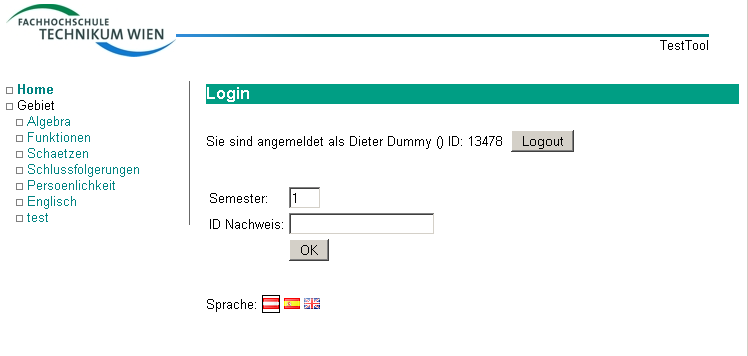
\includegraphics[width=0.75\textwidth]{testtool_login2.png}
	\caption{Testtool Einstellungen}
	\label{Testtool Einstellungen}
\end{figure}

In der folgenden Seite kann das Semester ausgew�hlt werden, f�r das der Reihungstest absolviert werden soll. Dies wird automatisch mit den Informationen aus dem FAS bef�llt und sollte in der Regel richtig bef�llt sein.\\
Im Unteren Teil, kann die Sprache ausgew�hlt werden, in der die Fragen und Vorschl�ge angezeigt werden. Diese Option steht nur dann zur Verf�gung, wenn beim Studiengang das Attribut testtool\_sprachwahl gesetzt ist. Standardm��ig ist die Sprache des Studienganges vorausgew�hlt.\\

\section{Starten eines Gebiets}

Im linken Men� scheinen nun die zugeteilten Gebiete auf.\\

\achtung{Wenn eines der Gebiete rot markiert ist, dann befinden sich Fehler in der Zusammenstellung des Gebietes. In diesem Fall starten Sie die Pr�fung in der Adminseite und beheben Sie die angezeigten Fehler.}\\
\\
\\
Beim Anklicken des Gebietes wird die Infoseite des Gebietes angezeigt (Frage mit der Nummer 0). Mit einem klick auf 'weiter' k�nnen die Demos zu diesem Gebiet angezeigt werden.\\
\\
Um das Gebiet zu starten, dr�cken Sie rechts oben auf 'Start'. Sobald das Gebiet gestartet ist, beginnt auch die Zeit zu laufen. Wenn die Zeit abgelaufen ist, wird das Gebiet automatisch beendet.

\begin{figure}
	\centering
	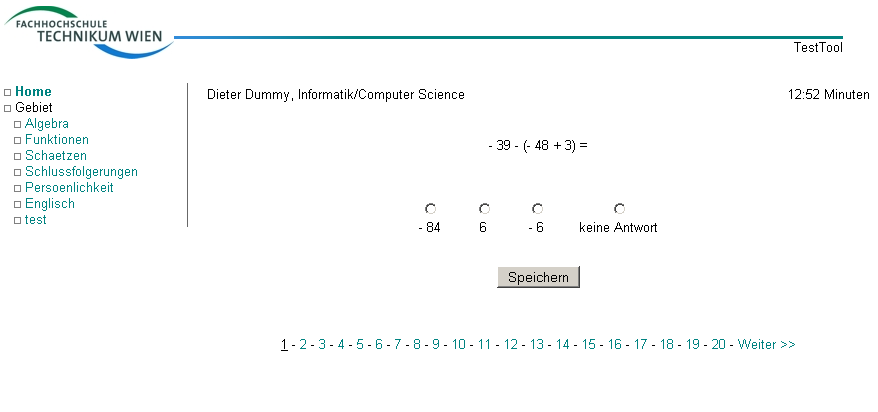
\includegraphics[width=0.75\textwidth]{testtool_frage.png}
	\caption{Beantworten von Fragen}
	\label{Beantworten von Fragen}
\end{figure}

Es werden nun nacheinander die Fragen angezeigt. Um die Frage zu beantworten markieren sie die Antwort und dr�cken auf Speichern. Nach dem Speichern wird automatisch die n�chste Frage angezeigt.


\chapter{Auswertung}

Nach erfolgreichem Abschluss des Reihungstests, kann die Auswertung gestartet werden. Klicken Sie hierzu auf der Administratorseite rechts oben auf 'Auswertung'.\\
\\
Hier kann der entsprechende Reihungstest und Studiengang ausgew�hlt und die Auswertung erstellt werden.\\

\begin{figure}
	\centering
	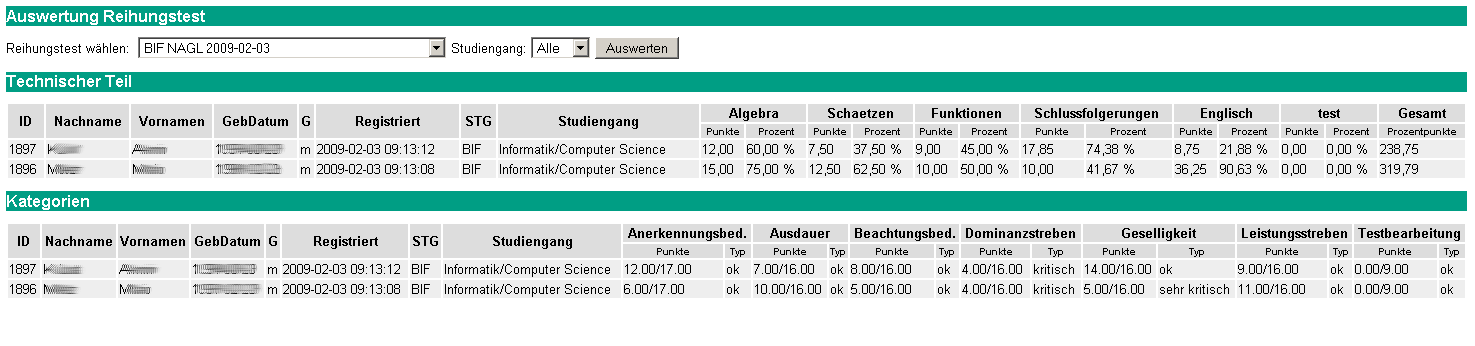
\includegraphics[width=0.75\textwidth]{testtool_auswertung.png}
	\caption{Auswertung des Reihungstests}
	\label{Auswertung des Reihungstests}
\end{figure}
\section{�bernehmen der Punkte ins FAS-Online}

Es gibt mehrere M�glichkeiten die Reihungstestpunkte ins FAS-Online zur �bernehmen:\\
\\
\begin{itemize}
\item Punkte einer einzelnen Person direkt im FAS abfragen
\item Punkte aller Personen eines Reihungstests ins FAS �bertragen
\item Punkte einer einzelnen Person aus der Reihungstestverwaltung �bertragen
\end{itemize}

\subsection{Punkte einer einzelnen Person direkt im FAS abfragen}

Im FAS k�nnen �ber den Karteireiter Prestudent, die Reihungstestpunkte einer einzelnen Person �bertragen werden. Klicken sie hierzu auf das Symbol neben dem Punkt Punkte1 im Abschnitt Reihungstest um die Punkte zu holen.

\begin{figure}
	\begin{center}
    \begin{picture}(100,51)
			\put(20,0){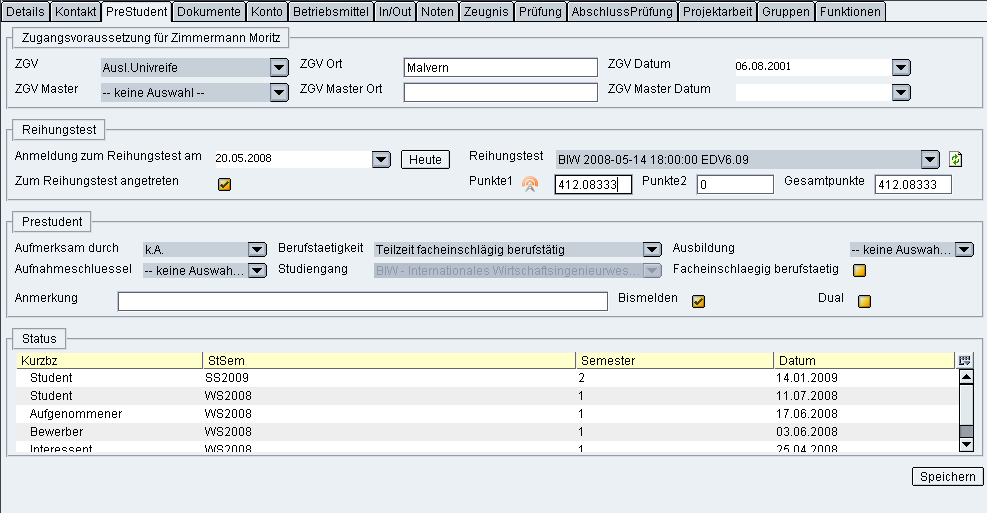
\includegraphics[height=51mm, width=100mm]{FAS_Prestudent1.png}}
			\markier{1}{68}{38}{1}{-1}
		\end{picture}
    \caption{�bertragen der Punkte}
		\label{�bertragen der Punkte}
  \end{center}
\end{figure}

Sie m�ssen anschlie�end auf Speichern dr�cken damit die Punkte gespeichert werden.\\
\\
\\
\\

\subsection {Punkte aller Personen eines Reihungstests ins FAS �bertragen}

�ber den Men�punkt Extras->Reihungstestverwaltung im FAS gelangen Sie zur �bersichtsseite �ber die vorhandenen Reihungstests. Wenn Sie einen Reihungstest ausw�hlen der bereits abgeschlossen ist, erhalten sie die M�glichkeit �ber den Link 'alle Punkte ins FAS �bertragen' die Punkte aller Personen dieses Reihungstests ins FAS zu �bertragen.

\begin{figure}
	\begin{center}
    \begin{picture}(100,51)
			\put(20,0){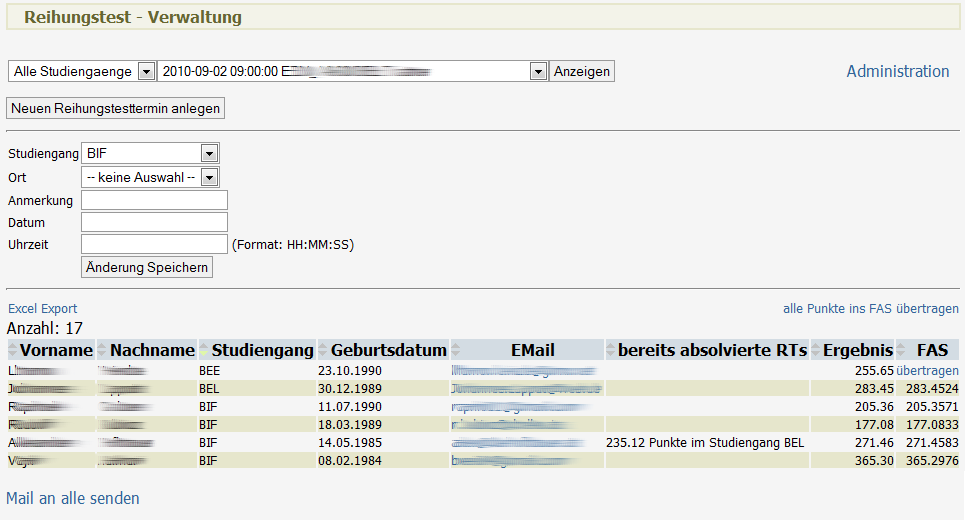
\includegraphics[height=51mm, width=100mm]{FAS_Reihungstest1.png}}
			\markier{1}{97}{27}{1}{-1}
		\end{picture}
    \caption{�bertragen der Punkte}
		\label{�bertragen der Punkte}
  \end{center}
\end{figure}

\subsection{Punkte einer einzelnen Person aus der Reihungstestverwaltung �bertragen}

�ber die Reihungstestverwaltung k�nnen Sie auch die Punkte einzelner Personen ins FAS �bertragen wenn Sie auf den Link '�bertragen' klicken.


%% Kapitel Ende   %%%%%%%%%%%%%%%%%%%%%%%%%%%%%%%%%%%%%%%%%%%%%%%%%


\appendix							% Beginn des Anhangs
\chapter{Schluss}


\end{document}
